\section{U-net:模型与原理}
\begin{frame}[allowframebreaks]
  \frametitle{\textsc{目录}} \vspace{-0.3cm}
    \begin{spacing}{0.0}
        \tableofcontents[currentsection,hideallsubsections]
    \end{spacing}   % 若不想要目录, 注释掉该句
\end{frame}



\begin{frame}
    \noindent\large\textbf{U-net}

    \vspace{1em}
    U-net首次提出是在2015年的MICCAI会议上,此后成为了图像分割任务的baseline,
    主流的图像分割模型大多遵循U-net的基本框架。

    \begin{figure}
        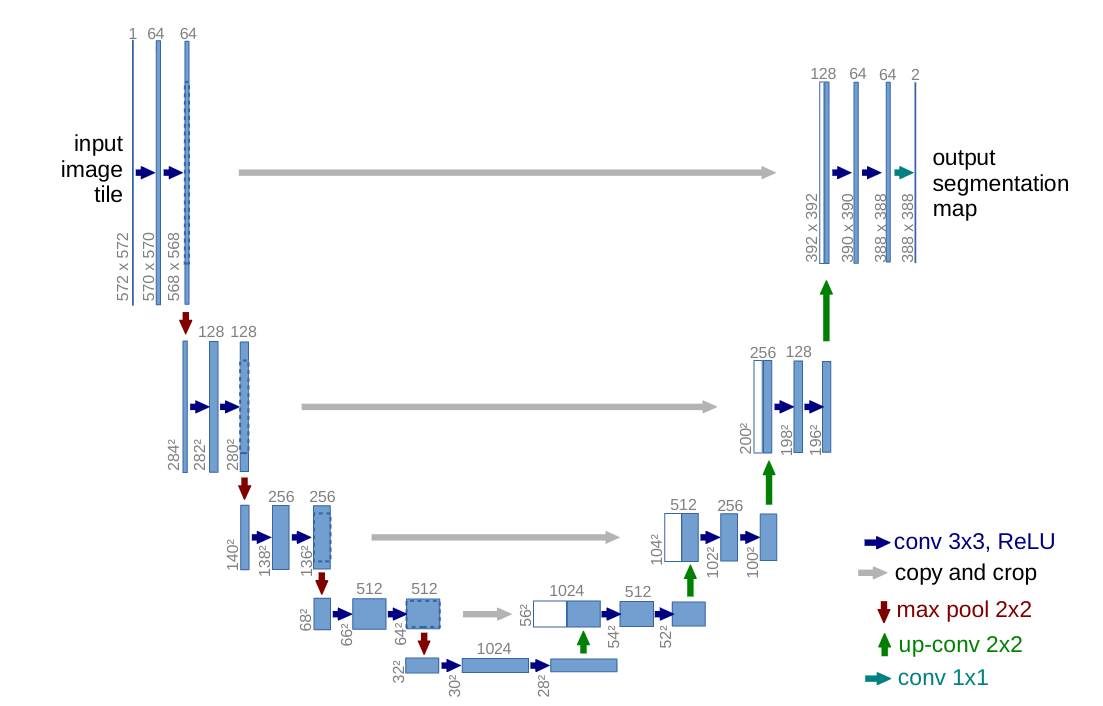
\includegraphics[width=9.5cm]{6.png}
    \end{figure}
\end{frame}

\begin{frame}
    \noindent\large\textbf{无缝分割策略}

    \vspace{1em}
    %U-net首次提出是在2015年的MICCAI会议上,此后成为了图像分割任务的baseline,
    %主流的图像分割模型大多遵循U-net的基本框架。

    \begin{figure}
        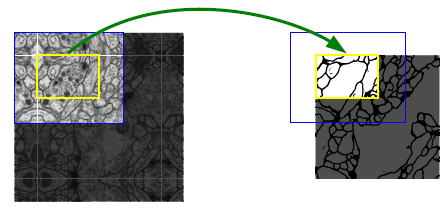
\includegraphics[width=9.5cm]{overlapTile.png}
    \end{figure}
\end{frame}

\begin{frame}
    \noindent\large\textbf{处理流程}

    \vspace{1em}
    \begin{figure}
        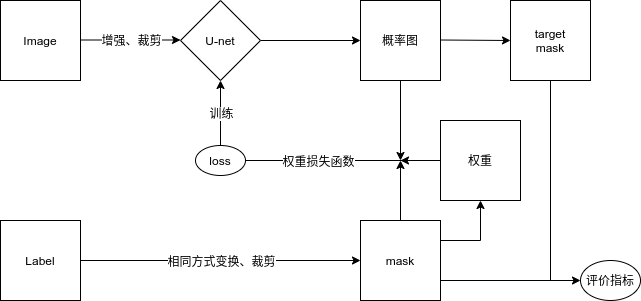
\includegraphics[width=10cm]{10.png}
    \end{figure}
\end{frame}

\begin{frame}
    \noindent\large\textbf{U-net为什么有效}

    \vspace{1em}
    $\bullet$ 跳跃连接保留了更多细节

    \vspace{1em}
    $\bullet$ 多层次特征图能够学习语义特征

    \vspace{1em}
    $\bullet$ 多层次特征融合既能保留细节又能学习语义

    \begin{figure}
        \centering
        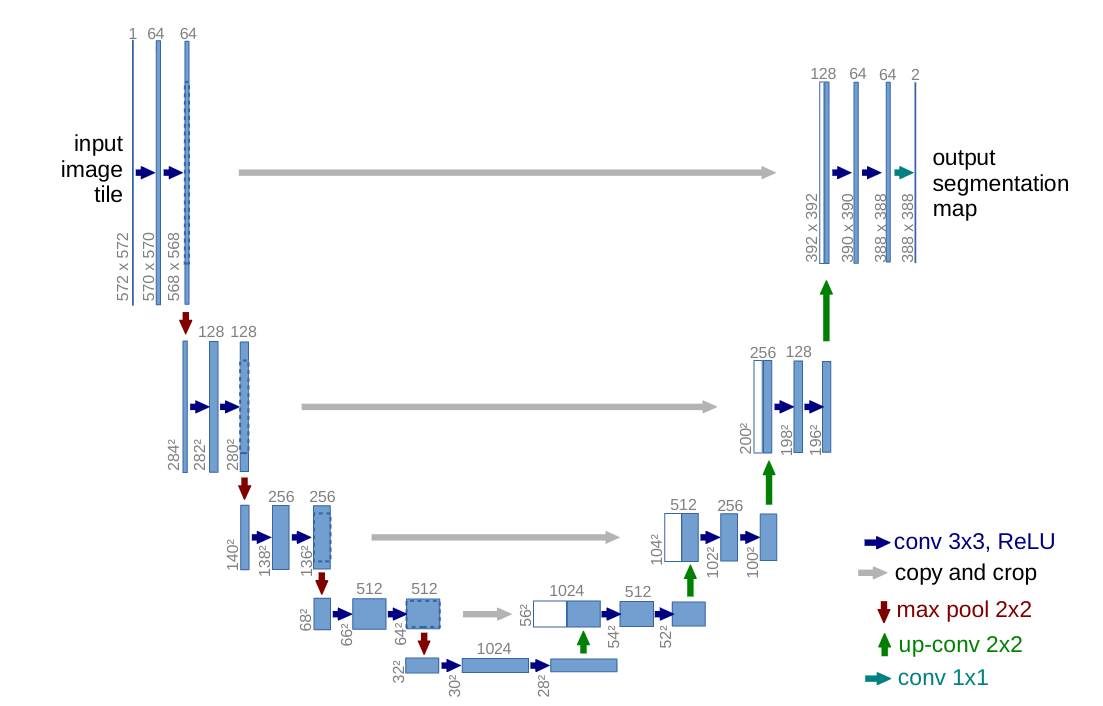
\includegraphics[height=5cm]{6.png}
    \end{figure}


\end{frame}

\begin{frame}
    \noindent\large\textbf{上采样方法}
    \vspace{1em}

    $\bullet$ 采样(线性插值、三次插值、最临近等)

    \begin{figure}
        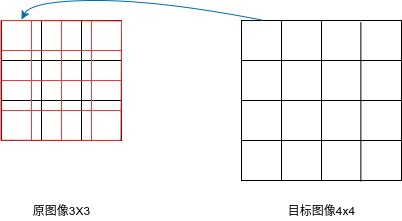
\includegraphics[width=8cm]{8.png}
    \end{figure}

    $\bullet$ 转置卷积(反卷积)
    \begin{figure}
        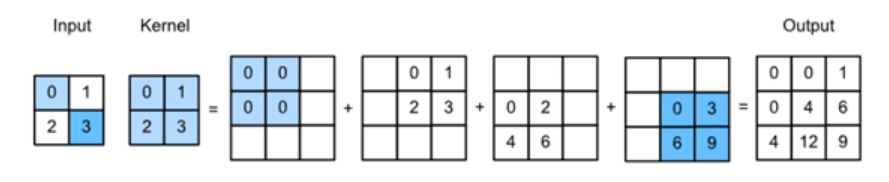
\includegraphics[width=11cm]{7.png}
    \end{figure}

\end{frame}

\begin{frame}
    $\bullet$ 上池化

    \begin{figure}
        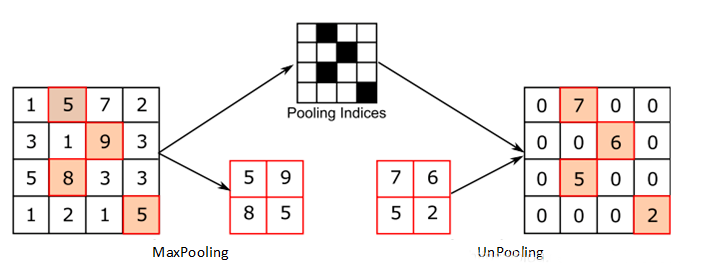
\includegraphics[width=11cm]{9.png}
    \end{figure}

    \vspace{1em}
    在pytorch的MaxPool操作当中,可以选择输出选取的位置,
    而MaxUnPool操作需要特征图和位置作为输入
\end{frame}

\begin{frame}[fragile]
    \begin{lstlisting}
# 采样
torch.nn.functional.interpolate()
torch.nn.functional.grid_sample()
torch.nn.functional.upsample()
torch.nn.UpsamplingBilinear2d
torch.nn.UpsamplingNearest2d
torch.nn.Upsample
# 转置卷积(反卷积)
torch.nn.ConvTranspose2d
torch.nn.functional.conv_transpose2d()
# 上池化
torch.nn.MaxUnpool2d
torch.nn.functional.max_unpool2d()
    \end{lstlisting}
\end{frame}

\begin{frame}

    \vspace{-5em}
    \noindent\large\textbf{特征图融合方法}


    \normalsize
    \vspace{1em}
    $\bullet$ 拼接:在通道维度上将特征图拼接起来

    \vspace{1em}
    $\bullet$ 相加:把相同形状的特征图直接相加

    \vspace{1em}
    区别:拼接不需要通道数一致但需要图尺寸相同,而相加需\\
    \quad \quad \quad 要通道数和图尺寸保持一致

    \vspace{1em}
    联系:相加可以看作是特殊的拼接,因为通常在拼接后会使用\\
    \quad \quad \quad$1\times1$卷积进行加权

\end{frame}

\begin{frame}
    \noindent\large\textbf{特征图融合方法}

    \vspace{1em}
    U-net首次提出是在2015年的MICCAI会议上,此后成为了图像分割任务的baseline,
    主流的图像分割模型大多遵循U-net的基本框架。

    \begin{figure}
        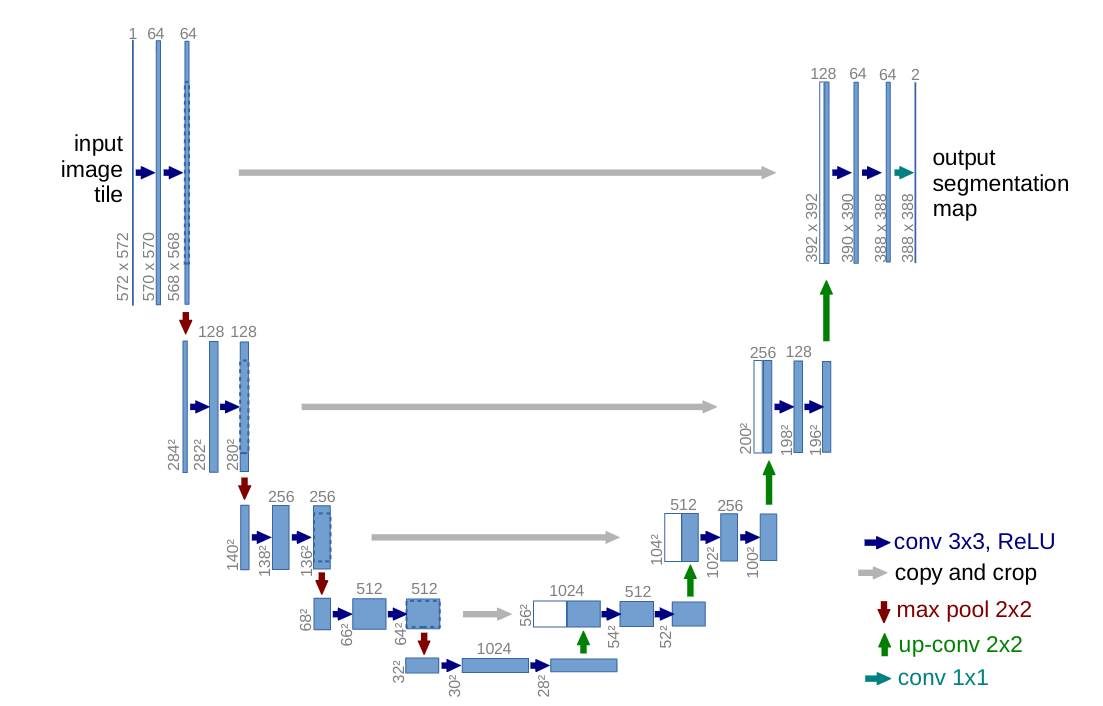
\includegraphics[width=9.5cm]{6.png}
    \end{figure}
\end{frame}

